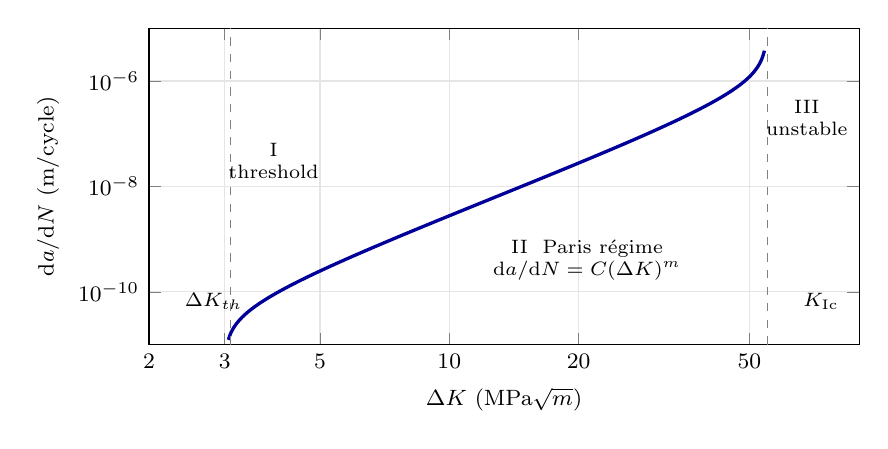
\begin{tikzpicture}
\begin{loglogaxis}[width=10.6cm,height=5.6cm,xlabel={$\Delta K$ (MPa$\sqrt{\text{m}}$)},ylabel={$\mathrm{d}a/\mathrm{d}N$ (m/cycle)},
 xmin=2,xmax=90,ymin=1e-11,ymax=1e-5,grid=both,grid style={gray!20},
 xtick={2,3,5,10,20,50},xticklabels={2,3,5,10,20,50},
 label style={font=\footnotesize},tick label style={font=\footnotesize}]
\addplot[very thick,blue!60!black,domain=3.06:54.2,samples=400]
  {3e-12*x^3*sqrt(1-3/x)/sqrt(1-x/55)};
\draw[gray,dashed] (axis cs:3.1,1e-11) -- (axis cs:3.1,1e-5);
\draw[gray,dashed] (axis cs:55,1e-11) -- (axis cs:55,1e-5);
\node[font=\scriptsize,anchor=south west] at (axis cs:2.3,3e-11) {$\Delta K_{th}$};
\node[font=\scriptsize,anchor=south east] at (axis cs:85,3e-11) {$K_{\mathrm{Ic}}$};
\node[font=\scriptsize,align=center] at (axis cs:3.9,3e-8) {I\\ threshold};
\node[font=\scriptsize,align=center,anchor=west] at (axis cs:12,4e-10) {II\ \ Paris r\'egime\\ $\mathrm{d}a/\mathrm{d}N=C(\Delta K)^m$};
\node[font=\scriptsize,align=center] at (axis cs:68,2e-7) {III\\ unstable};
\end{loglogaxis}
\end{tikzpicture}